\documentclass{article}

% if you need to pass options to natbib, use, e.g.:
% \PassOptionsToPackage{numbers, compress}{natbib}
% before loading nips_2017
%
% to avoid loading the natbib package, add option nonatbib:
% \usepackage[nonatbib]{nips_2017}

\usepackage[final]{nips_2017}

% to compile a camera-ready version, add the [final] option, e.g.:
% \usepackage[final]{nips_2017}

\usepackage[utf8]{inputenc} % allow utf-8 input
\usepackage[T1]{fontenc}    % use 8-bit T1 fonts
\usepackage{hyperref}       % hyperlinks
\usepackage{url}            % simple URL typesetting
\usepackage{booktabs}       % professional-quality tables
\usepackage{amsfonts}       % blackboard math symbols
\usepackage{nicefrac}       % compact symbols for 1/2, etc.
\usepackage{microtype}      % microtypography
\usepackage{graphicx}
\usepackage{caption}
\usepackage{float}

\title{Machine Learning Project - Stock Fluctuations}

\author{
  Mary Letey \\
  \And
  Morgan Allen \\
  \And
  Colton Williams \\
  \And
  Aniq Shahid 
}

\begin{document}

\maketitle

\begin{abstract}
  Research project investigating relationships between media concerning companies and the aforementioned company's stock price. Theoretically, the stock price of a company is based in part on public perception of their market. This perception can easily be affected by media sources. The project team hypothesizes that social media sources and news sources may be used to predict daily stock price fluctuations within the technology industry. \textbf{TODO :: One sentence on results}.
\end{abstract}
 
\section{Introduction}

Stock prices generally appear unpredictable; however, \emph{theoretically} they are quite simple. Considering the most basic supply-demand model in economics, stock prices are functions of the supply and demand for ownership in a company. Because the "consumers" in this supply and demand model are viewing a stock as an investment, demand represents confidence in the performance of the company. Furthermore, an increasing stock price represents increased confidence in the potential of the company. Thus the stock price may be affected by a change in the public's understanding of a company's perceived growth and risk. Forms of media, such as news articles, may have a significant impact in these perceptions.

\begin{figure}[H]
    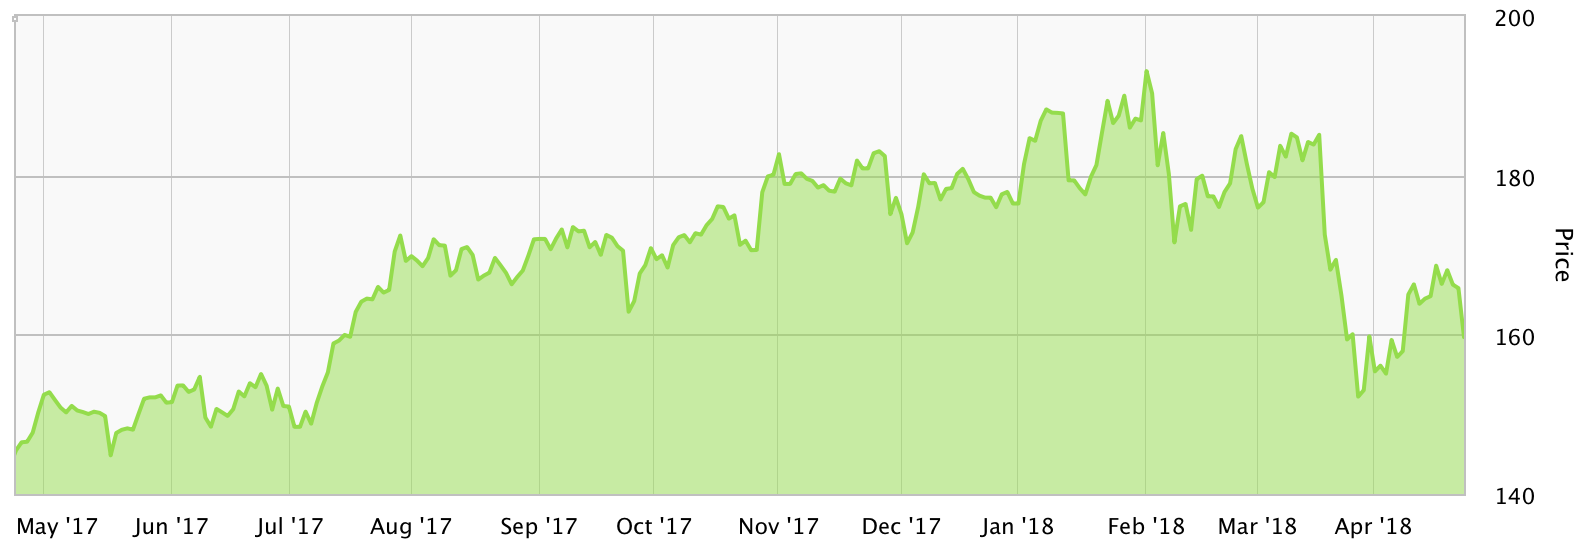
\includegraphics[scale=0.5]{FacebookYear.png}
  \caption{Facebook Stock Price \\
  \small Facebook stock price figure showing drastic decline at the beginning of April}
  \label{fig:faceplant}
\end{figure}

The most prominent feature in Figure \ref{fig:faceplant} is the dramatic drop around the beginning of April. Mark Zuckerburg testified before congress on April 8th. This hearing caused concern about Facebook's future, where traders expected Facebook's stock price to continue declining around a window of April 8th, according to Business Insider [1].

This project will examine the extent to which media sources affect stock prices, and how well media data affects stock price changes.

\newpage 

\section{Methods}

The focus of this project is to investigate the effects of media on stock price changes inside the technology industry. A single industry was chosen in order to maintain consistent results. The companies in this project representing the tech industry are [2]: \\
\\
1. Hewlett Packard \\
2. IBM \\
3. Seagate \\
4. Western Digital \\

The main media data is textual data from news articles into our model. The articles were gathered from reputable news sources, such as the Wall Street Journal. 

Furthermore, data from Google Trends is also included to obtain correlation between certain textual features to model public interest in the company.  

Numerical data measuring the closing price and volatility of shares was retrieved from Bloomberg. Other numerical data included macro-economic factors, such as the S\&P500, crude oil, and gold, in order measure a complete market change, as opposed to individual company changes. 

As a baseline model, a simple regression was used to establish a relationship between stock price and Google trends. The project team decided to use a simple model before adopting a more complicated model. We attempted achieving high accuracy results using a linear regression. However, we didn’t succeed in achieving highly accurate results; the error for predictions was quite high (more than 15\%). 

\textbf{TODO :: graph from aniq}

In order to begin analyzing text data, a logistic regression was used to model the impact of words on a binary, up-down change in the stock price.
The features were a bag-of-words derived from the the main bodies of the articles. The trained model predicted either 0 or 1, 0 being a stock decrease compared to the previous day, and 1 being an increase. 

To further analyze the article data we had gathered, we constructed a topic modeling algorithm that splits a company's articles into different classes based on content similarity. The goal of this step was to determine different themes occurring within articles. These topics were used as features in our main model. 

The main predictive model in this machine learning project is a Recurrent Neural Network (RNN). The RNN model has the capability to process high-throughput sequential data, such as the article data, as well as to tackle tasks with context spreading in time. In other words, as we were researching potential models, we learned that an RNN will be a good model since it uses sequences of prices as opposed to relying on just one input set for every output (closing stock price). These features of the RNN were very important to this project given that article content tends to build on previous articles. Additionally, the stock price on a given day is not only influenced by different factors on a particular day but a series of multiple days. 



\newpage
\section{Results}

\subsection{Linear Regression}

The Google Trends data provided an excellent starting point for this analysis. As one would expect, given that they measure public interest in a company, the Google Trends, when combined with previous stock data, was used in predicting the closing price of the company's shares. 

The Google Trends data combined with previous stock data when predicted the closing price of the company's shares. 

\begin{figure}[H]
	\centering
    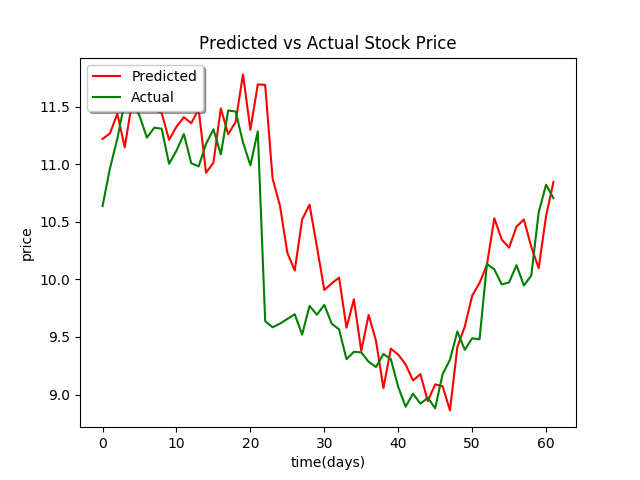
\includegraphics[scale=0.5]{googleHP.png}
  \caption{Prediction Results \\
  \small Graph showing predicted closing stock price versus actual value generated from a basic regression model for HP data}
  \label{fig:googlehp}
\end{figure}
For example, Figure \ref{fig:googlehp} shows almost exact results using a standard regression, where the Predicted and Actual curves are almost completely correlated. 

Unfortunately, the MSE of the regression model seemed to increase with additional data. This is quite contradictory to standard intuition, where error tends to decrease as the number of features increases. 

\begin{figure}[H]
	\centering
    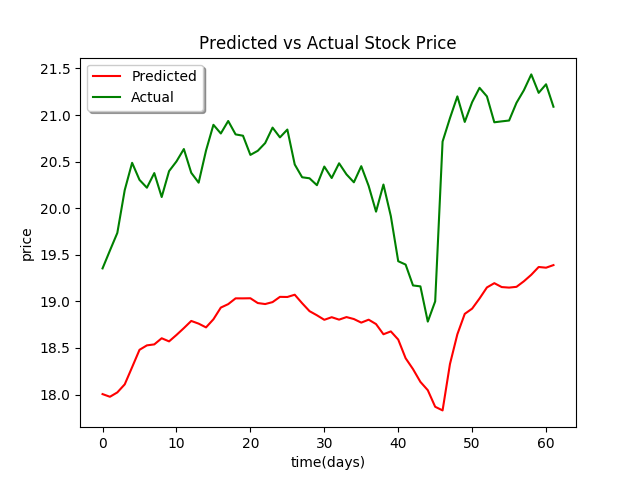
\includegraphics[scale=0.5]{googleIBM.png}
  \caption{Prediction Results \\
  \small Graph, using Google Trends, showing small covariance with large bias / error for IBM data}
  \label{fig:googleibm}
\end{figure}

Figure \ref{fig:googleibm} shows the large error for IBM, possibly as a result of overfitting. Techniques such as regularization and normalization were attempted, but to limited effectiveness. 

At a first glance, the errors in Table \ref{tab:linerrors} seem quite low. However, as mentioned in the introduction, the error behavior is not what we were looking for in the model. \\
\\
\\

{
 \centering
 \begin{tabular}{c | c}
 Company & MSE \\
 \hline
 HP & \\
 IBM & \\
 Seagate & \\
 Western Digital & \\
 \end{tabular}
 \captionof{table}{Average Investment Income \\
 \small Table of Mean Squared Error values generated by the logistic regression model with Google trends according to company}
 \label{tab:linerrors}
}



\textbf{TODO :: graphs}

\textbf{TODO :: desciption of regression error behavior}

\subsection{Logistic Regression}

The input features of the log-reg model was a bag-of-words derived from the article text data. It outputted either 0 or 1; 0 representing a decrease in the stock price compared to the previous day, and 1 representing an increase. The testing accuracy was moderately high as shown below. 

\textbf{TODO :: table}

Obviously, the table has no error listed for Western Digital. This points to a serious flaw in the logreg model. There is daily data for the closing stock price of a company; however, the article data is far from daily. In order to keep the input and output of the log-reg model compatible, any day where an article wasn't posted was dropped from the model. In other words, the only entries that were used were ones that had articles. This skewed our results, to the point where the data for Western Digital had no entries the the y-data that were 1. In other words, the accuracy of the Western Digital logreg model was 100\% because it would only predict zeros. 

This is a fundamental problem: An article from today might not predict the stock price today. There's a fundamental time delay in the relationship between stock price and articles. This realization was further motivation to use a sequential model, like an RNN. 

\subsection{Topic Modeling}

Coming up with novel approach to stock prediction is hard. Many people have tried, but very few have consistently done any better than the market. For our approach, we initially wanted to include text data from various sources which would accumulate to volumes more than any human brain could handle. The hope being that there is some predictive pattern buried in the data. To gather this data we built a web scraper to pull articles from \texttt{seekingalpha.com}, \texttt{fool.com} and \texttt{wsj.com}. We made an effort to gather data uniformly from the last five years, across the several different companies we were focused on. Despite the data challenge, we managed to collect several thousand articles.

Topic modeling is commonly used in Natural Language Processing (NLP) to reduce a large number of sparse features (like a bag-of-words model) into few dense and meaningful topics. For example, consider the following problem. Let’s suppose that our goal is to categorize an article into one of three categories. Fortunately, we have a large corpus of articles which already fall into one of these three categories. Unfortunately, none of these articles have been labeled with the category they belong to. One straightforward approach to solving this task could employ topic modeling.

Latent Dirichlet allocation (LDA) is a generative probabilistic model for collections of discrete data such as text corpora, and one of the most popular topic modeling techniques. LDA is applied to a bag of words representation of the text data, and applies a probability to each word indicating its likelihood of belonging to a specified number of topics. In regards to the above example, we would be able to inspect inspect the sorted probabilities of each of our three topics and be able to determine which category an article belongs to.

When we ran LDA on our corpus of scraped articles, topics like the following emerged:

\texttt{TODO :: insert colton's table}

Diverging from the simple example above, our purpose for these topics was not to classify the documents, but instead to use them to capture the original "theme" of the document in far fewer features. In our case we reduced the several thousand column wide bag-of-words representation into a 25 column wide topic representation. 

\texttt{TODO :: colton explain why 25 topics were chosen}

\subsection{Recurrent Neural Networks}

As far as the implementation goes, the inputs to the network include closing price, Google trends data, and topic modeling results of a given stock for each day in a \texttt{csv} file. Instead of using one input for each output, use sliding window of fixed size $n$, where features information for $n$ consecutive days is used as input and closing price for $n+1$ is used as output. In other words information from $n$ days is used to predict price for the $n+1^{th}$ day. This forms an unrolled version of an RNN and helps with faster back propagation through time training. Data from each company’s stock is used separately for training and testing purposes to analyze network’s performance on highly correlated data. For all our computations, we take at least 10\% of the data for training purposes. We didn’t take more than 20\% of the data for testing to ensure there is enough data for training purposes.

Regularized and normalized weights and data to prevent over-fitting the data, as well as faster learning. Performed data shuffling for better training accuracy.

\textbf{TODO :: graphs}

\textbf{TODO :: aniq writes error analysis}

\section{Discussion}

The team was able to flesh out a solid model, with low error rates. This model can easily be built upon to include more data sources, such as twitter and annual legal data. 

One of the biggest challenges was getting enough clean data from a variety of sources. Despite our efforts, there were often significant gaps in dates between published articles.

RNN’s are potentially a great tool for stock predictions, but they require a large amount of data to achieve maximum potential. In a low data situation, a generative model is one of the best choices. However, as more data is collected and the gaps are filled, the RNN accuracy will continue to improve and eventually outperform a generative model. 


\section{References}

\small

\subsection{Figures}

Figure \ref{fig:faceplant} from Yahoo Finance

Figure \ref{fig:googlehp} created by Aniq Shahid's tensorflow model. 

\subsection{Citations}

[1] Ciolli, Joe (2018, April 10) \emph{Facebook traders are bracing for the worst ahead of Mark Zuckerberg's hearing}. Retrieved from \url{http://www.businessinsider.com/facebook-stock-price-hedging-ahead-of-mark-zuckerberg-congressional-testimony-hearing-2018-4}

[2] We had originally used Dell as a 5th company, but unfortunately we ran into a data shortage for that company. We planned on swapping to Intel as a 5th company (included in the poster). However, we didn't have enough time to gather the data for another company. 

\end{document}
